Una volta affrontata l'interazione della radiazione con la materia, siamo pronti per discutere i rivelatori. Prima però di andare a discutere nel dettaglio le diverse tipologie di rivelatore, ne presentiamo alcune proprietà generali. Infatti, nonostante nel corso degli anni siano state sviluppate diverse tipologie di rivelatori che sfruttano meccanissimi diversi, hanno elettronica differente ecc., ci sono dei concetti di base che sono validi per tutti i rivelatori.

\section{Che cos'è un rivelatore}

Un rivelatore si può definire come uno strumento che viene usato per rivelare il passaggio di una particella o di una radiazione.

I rivelatori non sono tutti gli stessi, ce ne sono di diverse tipologie aventi diverse funzionalità ulteriori a quella di rivelare il passaggio di una particella: alcuni sono in grado di misurare l'energia della particella oppure tracciarla, quindi andare ad individuare il percorso seguito della particella o addirittura in alcuni casi identificarla, quindi capire che tipo di particella è passata attraverso di esso. Tuttavia, indipendentemente dalle diverse tipologie di rivelatori, è essenziale che un principio di base sia rispettato: affinché un rivelatore possa rivelare una particella o una radiazione, è fondamentale che queste interagiscano con il rivelatore stesso attraverso uno dei meccanismi che abbiamo discusso in base al tipo di particella o di radiazione che stiamo andando a considerare.

Come abbiamo studiato, l'interazione tra particelle e materiali dipende dalla sezione d'urto dei vari processi, che a sua volta è influenzata dalle caratteristiche della particella incidente e del materiale assorbitore. Per questo motivo, è essenziale comprendere come variano le sezioni d'urto nei diversi processi per capire le scelte progettuali dei rivelatori, come la geometria, i materiali utilizzati e le prestazioni ottenibili. Quando si progetta un rivelatore, bisogna considerare che, sebbene possa essere ottimizzato per rivelare certi tipi di particelle, ciò comporterà inevitabilmente delle limitazioni. Ad esempio, un rivelatore concepito per particelle cariche potrebbe non essere adatto per la radiazione elettromagnetica. Inoltre, il materiale con cui è costruito determinerà l'efficienza del rivelatore in relazione al tipo di particelle e alla loro energia.

Un aspetto fondamentale nella rivelazione è il \textit{tempo di interazione}. Questo rappresenta il tempo necessario per arrestare una particella o per lo sviluppo di uno sciame. I tempi di interazione sono estremamente brevi, dell'ordine dei nanosecondi nel caso di un materiale gassoso e dei picosecondi nel caso di un materiale solido. Oltre a questi, bisogna considerare anche il tempo che impiega il rivelatore per raccogliere il risultato dell'interazione, che chiaramente varia a seconda del meccanismo di interazione.

Il risultato netto dell'interazione delle radiazioni in un'ampia categoria di rivelatori è la comparsa di una determinata quantità di carica elettrica di ionizzazione $Q$ all'interno del volume attivo del rivelatore\footnote{Il volume attivo di un rivelatore è quella parte del rivelatore stesso in cui avviene l'effettiva rivelazione delle radiazioni, ovvero dove le particelle interagiscono con il materiale del rivelatore producendo segnali rilevabili, come la creazione di cariche elettriche, scintillazioni, o altri fenomeni misurabili.}. Successivamente, questa carica deve essere raccolta per formare il segnale elettrico di base. Tipicamente, la raccolta della carica viene realizzata attraverso l'imposizione di un campo elettrico all'interno del rivelatore, che provoca lo spostamento delle cariche positive e negative create dalla radiazione in direzioni opposte, producendo così un segnale in uscita. Il tempo necessario per raccogliere completamente la carica varia notevolmente da un rivelatore all'altro; in generale, questi tempi di rivelazione sono leggermente più lunghi rispetto ai tempi di interazione: vanno dai nanosecondi ai microsecondi, ma possono arrivare anche all'ordine del millisecondo nel caso di rivelatori molto lenti. Man mano che affronteremo i diversi tipi di rivelatore, esamineremo anche questi tempi di risposta, ovvero i tempi di rivelazione.

\section{Modi di operazione}

Il modo in cui operano la maggior parte dei rivelatori è quello di dare luogo a un segnale\footnote{Questo segnale nella pratica è un impulso di corrente. Nel seguito la professoressa parla di questi segnali come segnali di tensione, ma credo siano equivalenti data la legge di Ohm. In ogni caso, il Knoll ne parla in \S4.2.C\,.} ogni qualvolta vengono attraversati da una particella o da una radiazione. Fanno eccezione una classe di rivelatori che potremmo definire come rivelatori visualizzanti o traccianti, i quali funzionano semplicemente visualizzando il passaggio delle particelle, cioè permettono di visualizzare il passaggio di una particella senza però avere un segnale in uscita in corrispondenza del passaggio della particella o della radiazione. Degli esempi sono le emulsioni nucleari, che possiamo immaginarle come delle lastre fotografiche che visualizzano la traccia di una particella, oppure le camere a bolle e le camere a nebbia.

Concentriamoci sui rivelatori che segnalano il passaggio di una particella attraverso la formazione di un segnale elettrico.

\begin{figure}[H]
   \centering
   \begin{tikzpicture}
      \draw[->] (0,0) -- (9,0) node[right] {$t$};
      \draw[->] (0,0) -- (0,4) node[above] {$i(t)$};
      \draw[thick, red] (0,0) -- (1,0) arc (-90:0:0.2cm) -- (1.2,1.3) arc (180:90:0.2cm) -- (1.8,1.5) arc (90:0:0.2cm) -- (2,0.2) arc (180:270:0.2cm) -- (3,0) arc (-90:0:0.2cm) -- (3.2,2.8) arc (180:90:0.2cm) -- (3.8,3) arc (90:0:0.2cm) -- (4,0.2) arc (180:270:0.2cm) -- (6,0) arc (-90:0:0.2cm) -- (6.2,1.8) arc (180:90:0.2cm) -- (6.8,2) arc (90:0:0.2cm) -- (7,0.2) arc (180:270:0.2cm) -- (8,0);
    \end{tikzpicture}
\end{figure}

Ogni segnale avrà caratteristiche specifiche. Innanzitutto, si manifesteranno a intervalli temporali variabili, cioè, a meno che non si tratti di un fenomeno periodico, i tempi tra un evento e il successivo saranno casuali. Ciè è dovuto al fatto che l'arrivo e la rilevazione di particelle emesse da una sorgente radioattiva sono fenomeni casuali governati dalla statistica di Poisson, il che implica che l'intervallo temporale tra due eventi consecutivi non è fisso, ma cambia di volta in volta. Ciononostante, questa variazione segue una distribuzione che ha un andamento esponenziale decrescente.

La distanza tra due eventi consecutivi può variare notevolmente a seconda del fenomeno che si sta studiando e del tipo di radiazione rivelata. Ad esempio, se si dispone di una sorgente quasi esaurita con un'attività molto bassa, i segnali potrebbero verificarsi con una frequenza molto bassa; al contrario, in altri tipi di fenomeni, la frequenza di conteggio potrebbe essere molto più elevata. Per questo motivo i modi in cui un rivelatore può operare sono principalmente due:

\begin{itemize}[leftmargin=0.5cm]
   \item \textit{Pulsed mode}: il rivelatore rivela singoli impulsi in quanto questi arrivano in tempi abbastanza distanziati l'uno dall'altro, per cui è possibile studiare l'arrivo della singola particella/radiazione. Un esempio di fenomeno che si studia utilizzando un rivelatore in pulsed mode è la misura dell'arrivo di particelle della radiazione cosmica mediante un contatore Geiger: ogni volta che arriva una particella, questo emette un bip e viene prodotto un segnale, quindi è possibile contare singolarmente i diversi impulsi.
   \item \textit{Current mode}: quando gli impulsi sono molto ravvicinati in tempo, quindi abbiamo un'alta frequenza di conteggi, il rivelatore non riesce più a distinguere tra i singoli impulsi e lavorerà nella cosiddetta current mode, cioè nella modalità corrente. Quello che si va a misurare in questa modalità è sostanzialmente una corrente media.
\end{itemize}

In laboratorio lavoreremo principalmente in pulsed mode.

Chiariamo meglio che cos'è un segnale. Per segnale si intende una differenza di tensione, che quindi può essere visualizzato grazie a uno oscilloscopio.

\begin{figure}[H]
   \centering
   \includegraphics[width=0.7\textwidth]{immagini/segnali_rivelatori.png}
\end{figure}

Nella figura è mostrata la schermata di un oscilloscopio digitale, che consente di visualizzare più segnali contemporaneamente. Sull'asse orizzontale viene rappresentato il tempo, in quello verticale la tensione.

In questo caso, sono rappresentati due segnali distinti: uno in giallo e uno in rosa. Questi segnali, pur essendo molto diversi tra loro, hanno in comune la caratteristica di essere impulsi. Si nota infatti come, a partire da un valore di tensione costante (detto baseline), si verifichi una variazione nella tensione che persiste per una certa durata. Successivamente, il valore della tensione ritorna al livello iniziale.

Pur essendo questa caratteristica comunque ad entrambi i segnali, essi sono molto differenti. Il segnale giallo è un segnale analogico, la cui ampiezza può variare in modo continuo. Attualmente stiamo osservando un impulso specifico, ma un futuro impulso, causato da una nuova particella o radiazione, potrebbe avere un'ampiezza leggermente diversa, mantenendo però la stessa forma generale. Ciò che cambia è l'ampiezza del segnale, ossia la distanza tra la baseline e il valore massimo raggiunto. Questa ampiezza può quindi assumere valori differenti in modo continuo.

Al contrario, il segnale rosa ha una forma completamente diversa: è squadrato (onda quadra) e ha una durata che, in questo caso, viene spesso determinata dall'utente o dall'elettronica utilizzata. In questo contesto, non ci concentriamo sulla durata del segnale, ma piuttosto sul fatto che esso passa dalla baseline a un livello di tensione diverso, per poi ritornare alla baseline. Ad esempio, osservando la scala verticale, ogni divisione corrisponde a 200 mV, quindi questo segnale ha un'ampiezza di poco più di 800 mV. Si tratta di un segnale logico, che trasmette un'informazione limitata: indica semplicemente il passaggio dallo stato logico 0 allo logico 1, ma non fornisce altre informazioni. Se un nuovo impulso dovesse arrivare, avrebbe le stesse caratteristiche, con la stessa durata e ampiezza. Questo tipo di segnale è utile solo per contare il numero di impulsi ricevuti, senza poter estrarre ulteriori informazioni.

\subsection{Informazioni dai segnali}

Esistono diversi tipi di rivelatori che generano segnali differenti. Alcuni producono segnali logici, mentre altri emettono segnali analogici che trasportano informazioni aggiuntive sulla particella che possiamo dedurre dalle sue caratteristiche. Vediamo cosa possiamo dedurre.

\vspace{0.2cm}\textbf{Ampiezza}

Per ampiezza dei segnali intendiamo il valore massimo di tensione raggiunto dal segnale rispetto alla baseline. Essa può essere diversa a seconda dell'energia della particella incidente. Esistono infatti rivelatori che generano segnali la cui ampiezza è proporzionale all'energia depositata nel rivelatore stesso, risultando in un segnale più ampio quanto maggiore è l'energia depositata all'interno del rivelatore.

\E da notare che l'ampiezza del segnale puà variare anche per effetto delle fluttuazioni statistiche derivanti da altri fenomeni o a causa del rumore, per cui si ottiene un segnale di ampiezza leggermente diversa per motivi non fisici, nel senso che non è stata realmente depositata un'energia di valore diverso.

\vspace{0.2cm}\textbf{Tempo di arrivo}

Esso è il tempo associato al segnale e che fornisce informazioni sul tempo di arrivo della particella. Per capire quando il segnale è effettivamente arrivato è sufficiente andare a vedere l'istante in cui il segnale si discosta dalla baseline. Nel caso riportato in figura, notiamo come per le prime quattro suddivisioni della scala dei tempi (corrispondenti ciascuna a 100 ns) non c'è un segnale, in quanto abbiamo una tensione che è costante. Dopodiché all'improvviso parte un segnale dovuto appunto ad un impulso. Quand'è che parte l'impulso? Non è facile determinare l'inizio di questo segnale perché ci sono delle leggere fluttuazioni dovute al rumore elettrico, infatti la linea della tensione non è esattamente costante, bensì fluttua anche quando non c'è nessun impulso. In casi come questi si deve scegliere una sorta di soglia, cioè un livello di tensione superato il quale si può ritenere abbastanza ragionevole che effettivamente si stia presentando un segnale e non si tratti semplicemente di una fluttuazione. In tal caso, il tempo di inizio del segnale sarà dato dall'istante in cui si supera tale livello di soglia.

\vspace{0.2cm}\textbf{Forma e durata}

Oltre all'ampiezza, ci può interessare anche quanto dura il segnale. Ad esempio il segnale giallo raggiunge il suo valore massimo all'incirca a 50 ns dal suo inizio, ma in realtà si esaurisce in 300 ns.

Ci può interessare anche la forma del segnale, ad esempio la discesa o la risalita. Infatti ci sono dei rivelatori che producono dei segnali che hanno forme diverse a seconda del tipo di particella che ha inciso, per cui a seconda che sia una particella carica o una radiazione elettromagnetica il segnale prodotto cambia forma e quindi se si è in grado di analizzare la forma del singolo segnale si può capire se il rivelatore ha misurato ad esempio una particella $\alpha$ o un $\gamma$ e quindi attraverso l'analisi della forma del segnale si può procedere a una sorta di identificazione, cioè capire effettivamente che particella è arrivata.

\section{Analisi delle ampiezze}

Nella maggior parte dei rivelatori che tratteremo, l'ampiezza ci darà informazioni sull'energia che sarà depositata dalla particella incidente sul rivelatore. Infatti, come abbiamo già detto, l'ampiezza del segnale dipenderà dall'energia depositata dalla particella/radiazione; nella maggior parte dei casi esiste una relazione lineare tra energia depositata e ampiezza del segnale prodotto, quindi se andiamo ad analizzare l'ampiezza del segnale in automatico sapremo quanta energia è stata depositata nel rivelatore. Questo processo equivale a fare un'analisi delle ampiezze, che tipicamente si fa rappresentando la distribuzione delle ampiezze degli eventi misurati. Solitamente tale distribuzione viene rappresentata mediante una distribuzione differenziale $\dv*{N}{H}$, che è sostanzialmente un istogramma degli impulsi misurati, detto \textit{spettro delle ampiezze}.

\begin{approfondimento}[Lo spettro degli impulsi]
   \footnotesize
   Questo approfondimento è dovuto al fatto che secondo me è spiegato molto male il concetto di distribuzione delle ampiezze, per cui riporto quanto detto dal Knoll in \S4.2 "Pulse height spectra".

   \vspace{0.2cm}La distribuzione delle ampiezze degli impulsi è una caratteristica del segnale in uscita di un rivelatore che viene comunemente utilizzata per dedurre informazioni sulla radiazione incidente o sul funzionamento del rivelatore stesso.

   Il modo più comune di rappresentare le informazioni sulle ampiezze degli impulsi è attraverso la distribuzione differenziale delle altezze degli impulsi. Una distribuzione ipotetica a scopo di esempio è mostrata nel seguente grafico:
   \begin{figure}[H]
      \centering
      \includegraphics[width=0.6\textwidth]{immagini/distribuzione_differenziale_ampiezze.png}
   \end{figure}
   Sulle ascisse sono riportate le ampiezze degli impulsi con scala lineare, che va da zero a un valore più alto dell'ampiezza di qualsiasi impulso osservato dalla sorgente; l'ordinata rappresenta il numero differenziale $\dd{N}$ di impulsi osservati con un'ampiezza all'interno dell'incremento differenziale di ampiezza $\dd{H}$, diviso per tale incremento, o $\dv*{N}{H}$. La scala orizzontale ha quindi unità di ampiezza degli impulsi (Volt), mentre la scala verticale ha unità di ampiezza inversa (Volt$^{-1}$).
   
   Il numero di impulsi la cui ampiezza si trova tra due valori specifici, $H_1$ e $H_2$, può essere ottenuto integrando l'area sotto la distribuzione tra questi due limiti, come mostrato nell'area tratteggiata in figura.

   \begin{equation*}
      \text{Numero di impulsi con ampiezza tra $H_1$ e $H_2$}
      =\int_{H_1}^{H_2} \dv{N}{H} \dd{H}
   \end{equation*}
   
   Il numero totale di impulsi $N_0$ rappresentato dalla distribuzione può essere ottenuto integrando l'area sotto l'intero spettro:
   \begin{equation*}
      N_0=\int_{0}^{+\infty} \dv{N}{H} \dd{H}
   \end{equation*}
   La maggior parte degli utenti degli strumenti di rivelazione è abituata a osservare la forma della distribuzione differenziale delle altezze degli impulsi per identificare caratteristiche significative della sorgente degli impulsi. L'ampiezza massima degli impulsi osservata (nel nostro esempio pari ad $H_5$) è semplicemente il punto lungo l'ascissa in cui la distribuzione arriva a zero. I picchi nella distribuzione, come quello per $H_2$, indicano ampiezze di impulsi intorno a cui si trovano molti impulsi; viceversa, le valli o i punti bassi nello spettro, come $H_3$, indicano valori dell'ampiezza degli impulsi intorno ai quali si verificano relativamente pochi impulsi.
   
   %L'interpretazione fisica dell'altezza dello spettro differenziale degli impulsi coinvolge sempre aree sotto lo spettro tra due limiti dati di altezza degli impulsi. Il valore dell'ordinata stessa ($\dv*{N}{H}$) non ha significato fisico fino a quando non viene moltiplicato per un incremento dell'ascissa $H$.
\end{approfondimento}

\begin{esempio}[Distribuzione delle ampiezze per il $^{\text{137}}$Ce]\label{es:distr_ampiezze_cesio}
   In figura possiamo vedere un istogramma delle ampiezze, ottenuto utilizzando uno scintillatore con una sorgente di \ce{^{137}Ce} che emette $\gamma$ monoenergetici a 662 keV.

\begin{figure}[H]
   \centering
   \includegraphics[width=0.615\textwidth]{immagini/distribuzione_ampiezze_impulsi_es_1.png}
\end{figure}

Quello che succede ad ogni interazione è che un $\gamma$ interagisce con il rivelatore, deposita una certa quantità della sua energia (che può essere tutta o anche solo una parte) e quindi in corrispondenza di ogni gamma si ottiene un segnale con una data ampiezza. Analizziamo allora questa distribuzione di ampiezze.

Se il $\gamma$ lasciasse ogni volta nel rivelatore tutta la sua energia, ci aspetteremmo di trovare sempre la stessa ampiezza, corrispondente nell'esempio a 662 keV. In realtà otteniamo uno spettro con una forma abbastanza complessa che ci dice che oltre a un valore di energia molto probabile e rappresentato dal picco in corrispondenza del canale 289, si presentano anche tanti eventi, quindi tanti $\gamma$, che rilasciano parte della loro energia, perché corrispondono a segnali di ampiezza più bassa. Il picco che vediamo è il cosiddetto picco fotoelettrico, cioè il picco che si ottiene quando il $\gamma$ interagisce per effetto fotoelettrico con lo scintillatore. Infatti in quel caso come prodotto dell'effetto fotoelettrico si ha un elettrone che ha assorbito tutta l'energia del fotone, il quale può percorrere pochi millimetri all'interno dell'elettrone prima di perdere tutta la sua energia. Quindi essenzialmente questi sono degli eventi in cui il gamma ha perso la sua energia per effetto fotoelettrico e l'ha trasferita all'elettrone e l'elettrone a sua volta rimane intrappolato all'interno del rivelatore perdendo tutta la sua energia attraverso i processi collisionali che abbiamo descritto in precedenza. In conclusione sono eventi in cui viene ricostruita tutta l'energia del $\gamma$ incidente. Ovviamente teoricamente dovremmo avere un delta di Dirac\footnotemark, ma nella realtà abbiamo un picco un po' più largo dovuto a effetti del rivelatore, che non è in grado esattamente di ricostruire l'energia con una precisione infinita, quindi abbiamo una sorta di risoluzione dettata dal rivelatore.

Tutti gli altri eventi che troviamo alla sinistra del picco, che prendono il nome di spalla Compton, corrispondono a dei casi in cui l'energia che viene rilasciata e depositata nello scintillatore è solamente una parte dell'energia del $\gamma$ incidente perché evidentemente sono avvenuti altri meccanismi\footnotemark. Si tratta infatti di effetti di scattering Compton, dove come prodotto finale si produce non solo un elettrone che chiaramente perderà la sua energia nello scintillatore, ma anche un fotone diffuso. Questo fotone ha una probabilità più bassa di interagire, quindi potrebbe fuggire dal rivelatore e non depositare la sua energia, ecco perché in questi eventi viene ricostruita solamente parte dell'energia che è quella dovuta all'elettrone scatterato durante l'effetto Compton. Abbiamo tanti valori di energia perché l'energia che viene assegnata al fotone diffuso e all'elettrone cambia a seconda dell'angolo di diffusione, quindi abbiamo uno spettro continuo di valori.

Chiaramente, se siamo interessati a sapere qual è l'energia del gamma, ci concentreremo sul picco fotoelettrico, in quanto corrisponde meglio all'energia del $\gamma$ di partenza.
\end{esempio}
\footnotetext[3]{I $\gamma$ corrispondono a transizioni tra livelli nucleari, per cui non possono assumere qualsiasi valore di energia bensì hanno dei valori per precisi, corrispondenti alla differenza energetica dei livelli tra cui avviene la transizione.}

\footnotetext[4]{Certamente non avvengono meccanismi di produzione di coppie perché stiamo parlando di gamma di 662 keV, quindi siamo al di sotto dell'energia di soglia.}

L'esempio appena visto ci mostra come il segnale che viene tradotto dal rivelatore possa fornire informazioni sull'energia depositata nel rivelatore. Ribadiamo che quest'ultima non corrisponde sempre all'energia della particella emessa, ma potrebbe essere soltanto una parte, a seconda dei meccanismi che si sono verificati all'interno del rivelatore.

Vediamo che tipo di informazioni si possono estrarre da uno spettro:

\begin{itemize}[leftmargin=0.5cm]
   \item Potremmo essere interessati a sapere quanti segnali sono arrivati complessivamente nel tempo di misura, in modo da valutare quante particelle siamo riusciti a misurare. Ovviamente questo numero è legato all'attività della sorgente, quindi più questa è attiva, maggiore sarà il numero di eventi che riusciamo ad accumulare in un dato intervallo di tempo, e questo si può valutare realizzando l'integrale dello spettro, quindi sommando sostanzialmente quanti eventi si trovano in ciascuno dei bin dell'istogramma;
   \item Potremmo essere interessati solamente a una pozione dello spettro, ad esempio potremmo voler analizzare soltanto gli eventi fotoelettrici, in modo da capire qual è la percentuale di eventi associati a tale fenomeno. Per fare ciò scegliamo degli estremi dello spettro e calcoliamo l'integrale dello spettro esteso solamente a tale regione;
   \item In base alla forma dello spettro possiamo individuare diverse regioni relative a particolari fenomeni, come nel caso della spalla Compton o del picco fotoelettrico. Inoltre possiamo andare a guardare il valore massimo delle ampiezze, quindi qual è la massima energia che viene misurata in questa tipologia di eventi.
\end{itemize}

\subsection{Calibrazione di uno spettro}

In laboratorio, un grafico del genere viene realizzato tramite un ADC, il quale traduce l'ampiezza del segnale in un numero che varia in un intervallo che dipende dal numero di bit a disposizione. Notiamo infatti come la distribuzione dell'\esref{es:distr_ampiezze_cesio} sia espressa in termini di canali, ossia in termini del numero prodotto dall'ADC. In particolare, nell'esperienza di laboratorio in cui adoperiamo uno scintillatore per misurare i $\gamma$ avremo a disposizione un ADC a 11 bit, il che vuol dire $2048$ numeri (da $0$ a $2047$). Nasce quindi la necessità di capire a che valore di energia corrisponde ciascun canale, e per fare ciò bisogna effettuare una calibrazione.

Per fare una calibrazione bisogna saper associare ciascun canale ad un valore di energia, quindi si utilizzano delle sorgenti note di cui conosciamo i valori di energia. Possiamo utilizzarne anche solamente due, come il cesio-137 che emette a 662 keV e il cobalto-60 che invece emette due $\gamma$ a due energie diverse, uno a 1117 keV e l'altro 1332 keV. La vicinanza di questi due valori fa sì che i due picchi fotoelettrici siano parzialmente sovrapposti, ma ciò è irrilevante in quanto ci interessa la possibilità di individuare il centroide del picco e di associarlo alla corretta energia.
\begin{figure}[H]
   \centering
   \includegraphics[width=\textwidth]{immagini/sorgenti_calibrazione.png}
\end{figure}
Adoperando queste due sorgenti avremo tre coppie di punti $\rm (canale, energia)$ relativi ai picchi fotoelettrici, per cui è possibile realizzare una procedura di best-fit per andare a individuare una retta di calibrazione come quella mostrata nella figura seguente:
\begin{figure}[H]
   \centering
   \includegraphics[width=0.6\textwidth]{immagini/retta_calibrazione_cesio_cobalto.png}
\end{figure}
Attraverso questa retta di calibrazione è possibile fare qualsiasi tipo di associazione; ad esempio, se abbiamo una sorgente che emette $\gamma$ con una data energia, attraverso la retta sappiamo a quale canale aspettarci il picco fotoelettrico. Viceversa, se abbiamo una sorgente incognita e vogliamo capire di che isotopo si tratta, andiamo a vedere i picchi e in base alla posizione di questi rispetto ai canali possiamo, mediante la retta di calibrazione, conoscere le energie e quindi capire qual è l'isotopo.

Il motivo per cui adoperiamo tale procedura per ottenere la calibrazione è che nella maggior parte dei casi la relazione tra la grandezza misurata e il canale è lineare. Purtroppo però non sempre la corrispondenza è lineare: a volte può essere lineare in una buona porzione dello spettro ma magari si presentano degli effetti di non linearità nelle regioni estreme (cioè nella regione a bassa ampiezza e in quella ad alta ampiezza), per cui è preferibile cercare di lavorare nella regione centrale dello spettro, dove la linearità è abbastanza assicurata.

\begin{esempio}
   In figura possiamo vedere un esempio di spettro ottenuto con un rivelatore al silicio per la misura di una sorgente $\alpha$ mista, cioè costituita da diversi isotopi, tant'è che abbiamo tre picchi di energia nota.
   \begin{figure}[H]
      \centering
      \includegraphics[width=0.7\textwidth]{immagini/esempio_calibrazione_spettro.png}
   \end{figure}
   Vediamo poi anche la corrispondente retta di calibrazione, ottenuta tramite best-fit. Idealmente la retta dovrebbe passare dallo zero degli assi, nella pratica ciò non avviene per effetti di non linearità. Per una calibrazione più accurata bisognerebbe avere anche delle sorgenti che corrispondono a energie più basse o più alte, in modo da andare a esplorare tutta regione di interesse. Ciononostante, anche con soltanto questa procedura si ottengono delle ottime calibrazioni.
   \begin{figure}[H]
      \centering
      \includegraphics[width=0.7\textwidth]{immagini/esempio_calibrazione_retta.png}
   \end{figure}
\end{esempio}

\subsection{Risoluzione in energia}

Osservando gli spettri visti finora notiamo come, sebbene teoricamente ci aspettiamo che siano mono-energetici, in pratica non lo sono. Abbiamo visto il caso dello spettro $\gamma$, in cui intervengono diversi meccanismi a complicare la situazione, ma anche nel caso della sorgente di particelle $\alpha$, le quali sono sempre mono-energetiche, in realtà non si ottengono dei picchi strettissimi. Quello che infatti ci saremmo aspettati è che, dato che le particelle hanno esattamente tutte la stessa energia, arrivando nel rivelatore e depositando tutta l'energia avrebbero prodotto sempre lo stesso segnale di uguale ampiezza; quello che invece notiamo è un allargamento del picco. Ciò è dovuto alla \textit{risoluzione energetica}, cioè alla capacità di un rivelatore di distinguere radiazioni che depositano nel rivelatore energie simili.

Immaginiamo di avere due radiazioni (sia radiazione elettro-magnetica che particelle cariche) che depositano nel rivelatore energie tra di loro molto simili. Quello che può succedere è che il rivelatore potrebbe non essere in grado di distinguere che si tratta di due energie effettivamente diverse, e ciò dipende da quanto vale la sua risoluzione in energia. Questa è una caratteristica dei rivelatori che misurano l'energia, e può essere stimata inviando sul rivelatore delle radiazioni monoenergetiche (ad esempio della radiazione $\alpha$, che sappiamo essere certamente monoenergetica, o utilizzando dei gamma monoenergetici) e misurando il corrispondente spettro in energia.
\begin{figure}[H]
   \centering
   \includegraphics[width=\textwidth]{immagini/risoluzione_in_energia.png}
\end{figure}
Quello che si osserva non è una delta di Dirac, dunque un istogramma che si costruisce solamente su un bin, bensì vediamo che gli eventi si suddividono su diversi bin, su diversi canali, proprio a causa di questo effetto di risoluzione energetica, quindi l'energia viene ricostruita con una certa precisione rispetto al valore vero.

Possiamo valutare la qualità nella ricostruzione dell'energia osservando la larghezza di questo picco. \E chiaro che più stretto è il picco, più il rivelatore sta lavorando bene in termini di misura dell'energia, cioè la misura dell'energia è più precisa. Il parametro che si valuta è la cosiddetta \textit{larghezza a metà altezza} del picco, che in inglese viene abbreviata con la sigla FWHM (Full Width Half Maximum). Questa rappresenta la larghezza del picco alla metà della sua altezza, per cui per trovarla bisogna vedere dove il picco raggiunge il valore massimo, dopodiché consideriamo la metà della sua altezza e andiamo a guardare che valori di ascisse si raggiunge in corrispondenza di questo. Questi due estremi individueranno la larghezza del picco metà altezza.

La risoluzione $R$ viene definita come la FWHM del picco divisa per il valore centrale di questo:
\begin{equation*}
   \text{Risoluzione}\equiv R=\frac{\text{FWHM}}{E_0}
\end{equation*}
Essendo definita come il rapporto tra due grandezze aventi entrambe le dimensioni di un'energia (la FWHM è un intervallo di energie e il denominatore è l'energia centrale del picco, cioè il suo centroide), la risoluzione risulta essere un numero puro, che si può eventualmente esprimere in percentuale. Per dare un'idea quantitativa, i rivelatori al silicio hanno una risoluzione dell'1\%, mentre gli scintillatori tra il 5\% e il 10\%.

Nella maggior parte dei casi, una buona approssimazione dei picchi che si ottengono negli spettri è quella Gaussiana, ossia è lecito immaginare che il picco abbia una forma Gaussiana\footnote{Tale approssimazione va bene soprattutto nella zona centrale, mentre le code potrebbero differire un po' da tale andamento.}. Sotto tale approssimazione, si può dimostrare che la larghezza a metà altezza può essere valutata conoscendo la deviazione standard della Gaussiana, infatti le due grandezze sono legate attraverso la relazione
\begin{equation*}
   \rm FWHM=2.35\sigma
\end{equation*}
\footnote{Questa parte l'ho presa dal Leo, \S5.3, \textit{"Energy Resolution. The Fano Factor"}.}La risoluzione in energia in realtà non è costante per un dato rivelatore. In generale, essa è una funzione dell'energia depositata nel rivelatore, in maniera tale che $R$ migliora con l'aumentare dell'energia. Cio è dovuto al fatto che i processi di ionizzazione ed eccitazione seguono delle statistiche di tipo Poissoniano o simile. Infatti, si scopre che l'energia media necessaria per produrre una ionizzazione è un valore fisso, $w$, dipendente solo dal materiale. Per una data energia depositata $E$, quindi, ci si aspetterebbe in media un numero di ionizzazioni $J$ pari a
\begin{equation*}
   J=\frac{E}{w} 
\end{equation*}
Pertanto, con l'aumentare dell'energia, aumenta anche il numero di eventi di ionizzazione, risultando in fluttuazioni relative minori.

Per calcolare le fluttuazioni è necessario considerare due casi.

\newpage

\textbf{Primo caso: la radiazione ha depositato parte della sua energia nel rivelatore}

Per un rivelatore in cui l'energia della radiazione non viene totalmente assorbita, si verificano delle fluttuazioni nell'energia depositata (e dunque negli eventi prodotti) in quanto da particella a particella varia la sequenza di urti all'interno del rivelatore. Il numero di reazioni che producono il segnale è dato da una distribuzione di Poisson, dunque la varianza è data da
\begin{equation*}
   \sigma^2 = J
\end{equation*}
dove $J$ è il numero medio di eventi prodotti, ovvero il numero medio di coppie elettrone-ione nel caso di ionizzazione. La dipendenza della risoluzione dall'energia può allora essere espressa come:
\begin{equation*}
   R
   =2,35 \cdot \frac{\sqrt{J}}{J}
   =2,35 \cdot \sqrt{\frac{w}{E}}
\end{equation*}
dove il fattore 2,35 collega la deviazione standard di una Gaussiana alla sua larghezza a metà altezza\footnote{Infatti tale ragionamento vale anche nel caso in cui si segua una distribuzione Gaussiana, in quanto la Poissoniana, per valori medi elevati, può essere approssimata con questa.} e al denominatore abbiamo messo il numero di eventi $J$ che si verificano. Pertanto, la risoluzione varia inversamente alla radice quadrata dell'energia.

\vspace{0.2cm}\textbf{Secondo caso: la radiazione ha depositato tutta la sua energia nel rivelatore}

Potremmo avere dei rivelatori abbastanza spessi da far sì che la particella si arresti all'interno del rivelatore, perdendo quindi completamente l'energia.

Stavolta l'energia depositata sarà sempre la stessa, dunque è un valore fisso e costante, mentre nel caso precedente l'energia depositata poteva fluttuare. Il numero totale di ionizzazioni che può avvenire e l'energia persa in ciascuna ionizzazione sono quindi vincolati da questo valore.

Statisticamente, ciò significa che gli eventi di ionizzazione non sono tutti indipendenti, quindi le statistiche di Poisson non sono applicabili. Fano fu il primo a calcolare la varianza in questa condizione e trovò che essa è data da
\begin{equation*}
   \sigma^2 = F \cdot J
\end{equation*}
dove $J$ è il numero medio di ionizzazioni prodotte e $F$ è un numero noto come \textit{fattore di Fano}. Il fattore $F$ è una funzione di tutti i vari processi fondamentali che possono portare a un trasferimento di energia nel rivelatore. Questo include tutte le reazioni che non portano a ionizzazione, come ad esempio le eccitazioni di fononi, ecc. È quindi una costante intrinseca del mezzo rivelatore. Teoricamente, $F$ è molto difficile da calcolare accuratamente poiché richiede una conoscenza dettagliata di tutte le reazioni che possono avvenire nel rivelatore.

In questo caso la risoluzione è quindi data da:
\begin{equation*}
   R
   =2,35 \cdot \frac{\sqrt{FJ}}{J}
   =2,35 \cdot \sqrt{\frac{Fw}{E}}
\end{equation*}
Se $F=1$, la varianza è la stessa di quella per una distribuzione di Poisson e ci riconduciamo al caso precedente. Questo sembra essere il caso degli scintillatori, tuttavia, per molti rivelatori come quelli a semiconduttori o a gas, $F<1$. Questo, naturalmente, aumenta notevolmente la risoluzione di questi tipi di rivelatori.

\vspace{0.2cm}Oltre alle fluttuazioni nella ionizzazione, numerosi fattori esterni possono influenzare la risoluzione complessiva di un rivelatore. Questo include effetti dall'elettronica associata come rumore, derive, ecc. Supponendo che tutte queste fonti siano indipendenti e distribuite come gaussiane, la risoluzione totale $E$ sarà data dalla somma in quadratura di tutti i contributi:
\begin{equation*}
   (\Delta E)^2
   =(\Delta E_{\rm det})^2 + (\Delta E_{\rm elect})^2 + \ldots
\end{equation*}

\begin{esempio}
   \begin{minipage}{0.395\textwidth}
      \begin{figure}[H]
         \centering
         \includegraphics[width=0.9\textwidth]{immagini/spettro_alpha_riv_silicio.png}
      \end{figure}
   \end{minipage}
   \begin{minipage}{0.6\textwidth}
      \vspace{0.3cm}In figura è riportato lo spettro in energia di particele $\alpha$ prodotte dalla reazione
      \begin{equation*}
         \ce{^7Li + ^3 He -> {\alpha} + ^6Li}
      \end{equation*}
      misurate com un rivelatore di silicio.
   
      Il picco indicato con $B$ ha larghezza a metà altezza pari 150 keV ed ha il suo centroide in corrispondenza di 10.9 MeV. La risoluzione risulta essere
      \begin{equation*}
         R(\%)=\frac{150 \cdot 10^3}{10.9 \cdot 10^6}=1.4\%
      \end{equation*}
   \end{minipage}
   
   \vspace{0.6cm}Un altro modo per ricavare i valori di risoluzione è quello di realizzare un fit gaussiano dei picchi. Di seguito ne è riportato un esempio con i valori ottenuti.

   \vspace{0.3cm}

   \begin{minipage}{0.5\textwidth}
      \begin{figure}[H]
         \centering
         \includegraphics[width=0.9\textwidth]{immagini/spettro_alpha_riv_silicio_fit_gaussiano.png}
      \end{figure}
   \end{minipage}
   \begin{minipage}{0.495\textwidth}
      \centering
      \begin{tabular}{c|c|c}
      FWHM & Centroide & $\begin{array}{c}
         \text{Risoluzione}\\
         \text{percentuale}
      \end{array}$\\[0.4cm]
      \hline
      &&\\[-0.3cm]
      $9.1845$ & $939.18 \pm 3.90$ & $0.977\%$\\[0.1cm]
      $8.5015$ & $1076.93 \pm 3.61$ & $0.789\%$\\[0.1cm]
      $9.1845$ & $1138.36 \pm 6.46$ & $1.336\%$\\[0.1cm]
      \end{tabular}
   \end{minipage}
\end{esempio}

\begin{esempio}
   Se volessimo ottenere risoluzioni migliori dell'1\%, è necessario ricorrere ad altra strumentazione. In particolare è preferibile utilizzare dei sistemi basati su spettrometri magnetici, cioè sistemi che adoperano dei campi magnetici per curvare le particelle e indirizzarle verso dei rivelatori e in base alla traiettoria seguita della particella si conosce l'energia. 

   In questo caso si può arrivare a risoluzioni molto più spinte, come possiamo vedere ad esempio nel seguente spettro di particelle $\alpha$, dove il picco $\alpha_{61}$ ha una larghezza di 2.5 keV ed un'altezza del picco di 5.97 MeV:
   \begin{figure}[H]
      \centering
      \includegraphics[width=0.7\textwidth]{immagini/spettro_alpha_riv_spettrometro.png}
   \end{figure}
   Svolgendo i conti, otteniamo che
   \begin{equation*}
      R(\%)=\frac{2.5 \cdot 10^3}{5.96 \cdot 10^6}=0.04\%
   \end{equation*}
   molto al di sotto del caso precedente.

   Che conseguenze avremmo avuto se la risoluzione fosse stata dell'1\%? Su un picco di 5.97 MeV, l'1\% corrisponde a $\rm 60 \; keV=0.06 \; MeV$, dunque l'ampiezza del picco sarebbe stata $\rm 5.97 \pm 0.06 \; MeV$. Se andiamo a guardare il grafico, notiamo come in tale range rientrino gli ultimi quattro picchi, i quali dunque verrebbero confusi dato che la risoluzione in energia non permetterebbe di distinguerli l'uno dall'altro. In altre parole, questi picchi sarebbe così larghi che andrebbero a sovrapporsi in unico picco, risultando così impossibile distinguerli.
\end{esempio}
\section{Efficienza di un rivelatore}
Analizziamo ora un altro aspetto dei rivelatori, ossia l'efficienza. Questo aspetto è particolarmente importante nel caso della misura di particelle neutre, le quali interagiscono con meccanismi diversi da quelli delle particelle cariche e che hanno inefficienze di rivelazione notevoli, quindi è molto importante conoscere le efficienze di rivelazione.
\subsection{Efficienza intrinseca di rivelazione}
Il concetto di efficienza intrinseca di un rivelatore vale per qualsiasi tipologia di rivelatore. Infatti non è detto che tutte le radiazioni/particelle che incidono sul rivelatore siano in grado di produrre un segnale misurabile. Pensiamo ad esempio ai $\gamma$, i quali potrebbero arrivare sul rivelatore ma non interagire: in questo caso il $\gamma$ viene perso, cioè non viene misurato. Un altro esempio può essere quello di una particella carica, che per qualche motivo deposita poca energia nell'attraversare un rivelatore e produce un segnale di bassa ampiezza, il quale può essere confuso con del rumore e non viene misurato.

Questi esempi ci mostrano come ci siano dei casi in cui il rivelatore risulta essere inefficiente. Proviamo allora a quantificare con una grandezza questa efficienza, che si dice intrinseca in quanto dipende dai meccanismi di interazione della radiazione con il rivelatore. L'efficienza intrinseca di un rivelatore $\varepsilon_{\rm int}$ è definita come
\begin{equation*}
   \varepsilon_{\rm int}
   =\frac{\text{n° particelle rivelate}}{\text{n° particelle incidenti}}
\end{equation*}

cioè come il numero di particelle che vengono rivelate, dunque che producono un segnale che viene in qualche modo acquisito, rispetto al numero di particelle che incidono di sul rivelatore.

Anche se concettualmente semplice, non è facile valutare l'efficienza intrinseca, perché questa dipende da tanti aspetti. In generale essa dipende
\begin{itemize}
   \item dal tipo di particella/radiazione;%, quindi potremmo ad esempio avere un rivelatore poco efficiente per la misura dei $\gamma$ ma molto efficiente per la rivelazione di particelle cariche come nel caso dei rivelatori a gas;
   \item dall'energia della particella, perché a seconda dell'energia intervengono dei meccanismi di interazione diversi;
   \item dal tipo di rivelatore;
   \item dal volume del rivelatore, in quanto in base alla sua grandezza la radiazione può fuoriuscire, non venendo quindi misurata.
\end{itemize}
  Tutti questi fattori rendono la valutazione dell'efficienza intrinseca un compito non semplicissimo, che spesso viene fatto infatti con dei codici di simulazione professionali che tengono conto di tutti i meccanismi di interazione.
  \subsection{Accettanza geometrica}
  Un altro fattore da considerare è la cosiddetta accettanza geometrica o efficienza geometrica. Questo è un concetto un po' diverso dal precedente, in quanto prima ci siamo posti il problema di capire se una particella che arriva a colpire il rivelatore viene rivelata o meno, adesso invece ci poniamo il problema di capire se una particella emessa da una sorgente arrivi a colpire o meno il rivelatore, indipendentemente dal fatto che poi, una volta intercettato il rivelatore, si formi un segnale.
  
  L'accettanza geometrica $\varepsilon_{\rm geo}$ è definita come il rapporto tra il numero di particelle incidenti sul rivelatore rispetto al numero di particelle emesse dalla sorgente:
  \begin{equation*}
   \varepsilon_{\rm geo}
   =\frac{\text{n° particelle incidenti}}{\text{n° particelle emesse dalla sorgente}}
  \end{equation*}
  \begin{esempio}[Sorgente puntiforme che emette particelle isotropicamente in tutto l'angolo solido]
      Immaginiamo di avere una sorgente puntiforme, posta ad una distanza $r$ da un rivelatore avente superficie $S$, che emette particelle in maniera isotropa, ossia con la stessa probabilità in tutte le direzioni dello spazio.
   \begin{figure}[H]
      \centering
      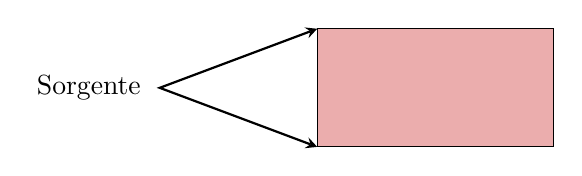
\begin{tikzpicture}
         \draw[fill=gray!40!red!40!] (0,0) rectangle (3cm, 1.5cm);
         %\draw[thick,-stealth] (-2,2) -- (1,0.5);
         \draw[thick,stealth-stealth] (0,1.5) -- (-2,0.75) -- (0,0);
         \node[left] at (-2,0.75) {Sorgente \quad};
      \end{tikzpicture}
   \end{figure}
   \E chiaro che se la particella viene ad esempio emessa nella direzione opposta al rivelatore non potrà mai colpirlo. Infatti, le uniche particelle che possono colpire il rivelatore sono quelle che intercettano l'angolo solido $\Omega$ sotteso da questo.
    
   L'accettanza geometrica si può allora valutare mediante un calcolo che dipende da caratteristiche puramente geometriche, infatti essa sarà data da
   \begin{equation*}
      \varepsilon_{\rm geo}=\frac{\Omega}{4\pi}
   \end{equation*}
   dove $4\pi$ è l'angolo solido totale di una sfera intera, ovvero l'angolo solido che corrisponde a tutte le possibili direzioni intorno a un punto. Spesso in fisica si parla di "rivelatori a $4\pi$", con cui si intendono rivelatori che vanno a circondare per intero la sorgente da cui possono essere prodotte delle particele.

   Se le dimensioni del rivelatore sono molto piccole rispetto alla distanza $r$, l'angolo solido può essere approssimato come
   \begin{equation*}
      \Omega \simeq \frac{S}{r^2}
   \end{equation*}
   e di conseguenza l'accettanza geometrica come
   \begin{equation*}
      \varepsilon_{\rm geo}=\frac{S}{4\pi r^2}
   \end{equation*}
   Per come è definita, $\varepsilon_{\rm geo}$ può variare da 0 (caso in cui l'angolo solido è nullo) a 1 (caso in cui l'angolo solido è $4\pi$). Se ad esempio avessimo un rivelatore capace di misurare tutte le particelle che vengono emesse alla destra della sorgente, allora avremmo una porzione di angolo solido pari $2 \pi$ e dunque un'efficienza geometrica pari a $0.5$.
\end{esempio}

\begin{esempio}[Angolo solido sotteso da un cilindro piano posto ad una distanza $\boldsymbol{r}$ da una sorgente puntiforme]\label{es:angolo_solido_riv_cilindro}
   Se abbiamo un rivelatore molto vicino alla sorgente, l'approssimazione utilizzata nell'esempio precedente non è più applicabile ed il calcolo dell'accettanza geometrica si complica. In tal caso, l'angolo solido sotteso dovrà essere valutato mediante la formula
   \begin{equation*}
      \Omega=\int_S \frac{\cos{\alpha}}{r^2} \dd{S}
   \end{equation*}
   dove $r$ rappresenta la distanza tra la sorgente e un elemento di superficie $\dd{S}$ e $\alpha$ è l'angolo tra la normale all'elemento di superficie e la direzione della sorgente.
   
   Consideriamo il caso in cui il rivelatore abbia forma cilindrica e la sorgente puntiforme sia posta sull'asse del cilindro
   \begin{figure}[H]
      \centering
      \begin{tikzpicture}[>=stealth,shorten >=1.8pt,shorten <=1.8pt,shape aspect=4]
         \node at (0,0) [thick,red!40!gray,cylinder, shape border rotate=90, draw,minimum height=3cm,minimum width=2cm,cylinder uses custom fill, cylinder end fill=gray!25!red!50!, cylinder body fill=gray!25!red!30!,rotate=90] {};
         \draw [thick,<->] (-1.4,1) -- (-4,0) node[left] {Sorgente \quad} -- (-1.4,-1);
      \end{tikzpicture}
   \end{figure}
   In tal caso, l'angolo solido sotteso del rivelatore è dato da
  \begin{equation*}
      \Omega=2\pi \qty( 1 - \frac{r}{\sqrt{r^2 + a^2}} )
  \end{equation*}
  dove $a$ è il raggio del cilindro.
\end{esempio}

\begin{esempio}[Angolo solido sotteso da un cilindro piano posto ad una distanza $\boldsymbol{r}$ da una sorgente estesa]
   Riprendiamo la configurazione dell'\esref{es:angolo_solido_riv_cilindro}, ma stavolta complichiamo il problema immaginando di avere una sorgente non più puntiforme bensì estesa, ad esempio avente la forma di un dischetto allineato con l'asse del rivelatore:
   \begin{figure}[H]
      \centering
      \begin{tikzpicture}[>=stealth,shorten >=1.8pt,shorten <=1.8pt,]
         \node at (0,0) [thick,red!40!gray,cylinder, shape border rotate=90, draw,minimum height=3cm,minimum width=2cm,cylinder uses custom fill, cylinder end fill=gray!25!red!50!, cylinder body fill=gray!25!red!30!,rotate=90,shape aspect=4] {};
         \draw [thick,<->] (-1.4,1) -- (-4,0) -- (-1.4,-1);
         \node at (-4,0) [thick,teal!40!gray,cylinder, shape border rotate=90, draw,minimum height=0.5cm,minimum width=1cm,cylinder uses custom fill, cylinder end fill=gray!25!teal!50!, cylinder body fill=gray!25!teal!30!,rotate=90,shape aspect=2] {};
         \node[above=1.5cm] at (-4.2,0) {Sorgente};
         \node[above=1.5cm] at (-0.2,0) {Rivelatore};
      \end{tikzpicture}
   \end{figure}
   In questo caso l'emissione di particelle può avvenire da qualsiasi punto della sorgente, per cui nell'espressione dell'angolo solido oltre l'integrazione vista prima se ne dovrà aggiungere una rispetto al volume della sorgente. Il problema qui in esame si risolve in maniera approssimata attraverso l'integrazione di funzioni di Bessel mediante metodi numerici (si veda Knoll \S4.VI). Solitamente però in situazioni del genere si preferisce adottare delle tecniche di simulazione Monte Carlo.
\end{esempio}

\subsection{Efficienza complessiva}
Una volta descritti questi due aspetti dell'efficienza, possiamo valutare l'efficienza complessiva del rivelatore. Infatti, il fatto che una particella venga effettivamente rivelata dipende da entrambi gli aspetti, in quanto dal punto di vista geometrico dipende dal fatto che la particella segue una traiettoria che va a intercettare il rivelatore e dal punto di vista strutturale dipende dal fatto che, una volta intercettato il rivelatore, effettivamente il segnale prodotto sia sufficientemente elevato da poter essere misurato.

In definitiva, l'efficienza complessiva è data semplicemente dal prodotto tra efficienza intrinseca ed efficienza geometrica:
\begin{equation*}
   \varepsilon_{\rm tot}
   \equiv \varepsilon
   =\varepsilon_{\rm geo} \cdot \varepsilon_{\rm int}
   =\frac{\text{n° particelle rivelate}}{\text{n° particelle emesse dalla sorgente}}
\end{equation*}
Da tale definizione segue che l'efficienza complessiva sia più piccola di entrambi i fattori.

\begin{esempio}[L'attività di una sorgente]
   Conoscendo l'efficienza complessiva, è possibile correggere i dati misurati per valutare le quantità originali. Cosa intendiamo con questa frase? Supponiamo di avere una sorgente in laboratorio di cui vogliamo misurare l'attività, cioè il numero di particelle emesse al secondo.

   Chiaramente per tale misura dovremo adoperare un rivelatore, ma il numero di particelle al secondo misurate da questo non coinciderà con l'attività della sorgente, perché noi misuriamo solo una porzione di tutte le particelle emesse, soltanto quelle che entrano nell'angolo solido sotteso dal rivelatore; inoltre non è detto che tutte le particelle che entrano nel rivelatore diano luogo ad un segnale e quindi vengano rivelate. Se tuttavia conosciamo l'efficienza complessiva, possiamo risalire all'attività andando a correggere la frequenza di conteggio ottenuta sperimentalmente dividendola per l'efficienza:
   \begin{equation*}
      \text{Attività}=\frac{\text{n° particelle/s misurate}}{\varepsilon}
   \end{equation*}
\end{esempio}

\section{Tempo di risposta}
Spesso si è interessati a conoscere il tempo di risposta di un rivelatore, che consiste nel tempo che impiega il rivelatore a formare il segnale. Tale informazione è utile in quanto il segnale che viene fornito può dare informazioni sul tempo di arrivo della particella/radiazione ed è dunque importante conoscere con che precisione viene fornito l'istante di arrivo della particella. In altre parole, siamo interessati alla \textit{risoluzione temporale}, la quale esprime l'indeterminazione nella conoscenza del tempo di arrivo.

La risoluzione temporale dipende da:

\begin{itemize}
   \item il tipo di rivelatore (a gas, scintillatore,ecc.);
   \item il modo di funzionamento del rivelatore;
   \item le dimensioni del rivelatore;
   \item l'elettronica associata per la trattazione del segnale.
\end{itemize}

\begin{esempio}[La misura del tempo di volo]
   Conoscere la risoluzione temporale è importante in diversi casi, ad esempio quando si effettuano delle misure di tempo di volo (spesso indicato con la sigla TOF, che sta per Time Of Flight) di una particella tra due rivelatori, che è una tecnica utilizzata per identificare le particelle e che consiste nel misurare il tempo che impiega una particella a percorrere una data distanza.

   Tale misura si realizza ponendo due rivelatori di cui conosciamo il tempo di arrivo in due posizioni ben precise e andando a misurare il passaggio di una particella che attraversa entrambi.
   \begin{figure}[H]
      \centering
      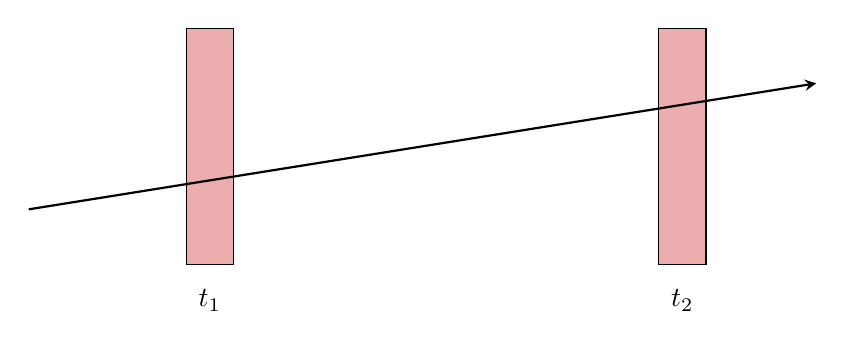
\begin{tikzpicture}
         \draw[fill=gray!40!red!40!] (0,0) rectangle ++(0.6cm, 3cm);
         \node[below=0.2cm] at (0.3,0) {$t_1$};
         \node[below=0.2cm] at (6.3,0) {$t_2$};
         \draw[fill=gray!40!red!40!] (6,0) rectangle ++(0.6cm, 3cm);
         \draw[thick,-stealth] (-2,0.7) -- (8,2.3);
      \end{tikzpicture}
   \end{figure}
   Il tempo di volo sarà dato dalla differenza tra questi due tempi e la risoluzione temporale complessiva di questa misura sarà data dalla somma in quadratura delle risoluzioni temporali dei due rivelatori
   \begin{equation*}
      \text{TOF}=t_2 - t_1
      \qqtext{,}
      \sigma_t=\sqrt{\sigma_{t,1} + \sigma_{t,2}^2}
   \end{equation*}
\end{esempio}

In molti casi è importante avere una buona risoluzione temporale, in quanto i tempi di volo sono molto brevi. Per dare un'idea, una particella che si muove a velocità prossima a quella della luce (30 cm/ns) percorrerà 1 m in un tempo dell'ordine dei nanosecondi. Di conseguenza la risoluzione temporale deve essere più piccola di questi valori, per cui bisogna saper scegliere bene che rivelatori adoperare. Tipicamente si ha che

\begin{itemize}
   \item Rivelatori a gas come camere a ionizzazione, contatori proporzionali, Geiger, ecc. producono segnali lenti (microsecondi) e hanno risoluzioni temporali scadenti;
   \item Rivelatori a gas di altro genere (Parallel Plate, MRPC, ecc.) hanno risoluzioni temporali estremamente buone (100 ps);
   \item Rivelatori basati su scintillatori di piccole dimensioni hanno risoluzioni dell'ordine del nanosecondo.
\end{itemize}

\section{Tempo morto}
L'ultimo aspetto che affrontiamo dei rivelatori riguarda il cosiddetto tempo morto. Infatti, ciascun sistema di rivelazione ha bisogno di un certo tempo per processare il segnale, e se durante questo tempo arriva un secondo evento quest'ultimo non verrà rivelato, venendo quindi perso. In altre parole, in una successione di eventi misurati da un rivelatore, esiste un tempo minimo tra due eventi successivi, al di sotto del quale il rivelatore non può separarli. Questo tempo è il tempo morto del sistema.

Se l'arrivo degli eventi è casuale, dunque segue la statistica di Poisson, poiché questa ha un andamento esponenziale decrescente è molto probabile che la differenza temporale tra due eventi sia piccola, dunque la probabilità che due eventi arrivino separati meno del tempo morto non è mai nulla. Una volta che però si conosce il tempo morto del sistema, si può andare a misurare soltanto quei fenomeni che hanno una frequenza di conteggio compatibile con il tempo morto del sistema, altrimenti perderemmo tanti eventi. Quindi, in base al tempo morto, si stabilisce il limite della frequenza di conteggio misurabile. Chiaramente l'ideale è avere una risposta veloce da parte dei rivelatori.

\subsection{Modelli per il comportamento del tempo morto}

Ci sono due modelli per descrivere il comportamento di un rivelatore dal punto di vista del tempo morto:

\begin{itemize}[leftmargin=0.5cm]
   \item \textit{Rivelatori non paralizzabili}, che sono dei rivelatori in cui un evento che accade durante il tempo morto non influenza ulteriormente il comportamento dei rivelatori.
   
   Possiamo immaginare schematicamente ciò che avviene nel rivelatore nella seguente maniera: se disponiamo gli eventi che avvengono (rappresentati dai rettangoli rosa) su un asse temporale, nel caso di rivelatore non paralizzabile il primo evento che arriva genera un certo processo nel rivelatore e di conseguenza l'elettronica processa il segnale, e tutto ciò richiede un certo tempo prima che si ripristinino le condizioni per una nuova rivelazione.
   \begin{figure}[H]
      \centering
      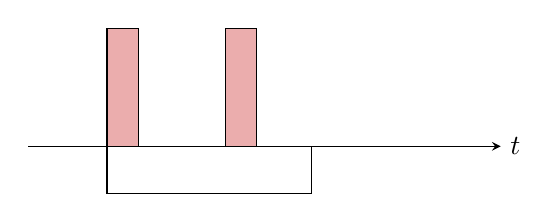
\begin{tikzpicture}
         \draw[-stealth] (0,0) -- (6,0) node[right] {$t$};
         \draw[fill=gray!40!red!40!] (1,0) rectangle ++ (0.4cm, 1.5cm);
         \draw[fill=gray!40!red!40!] (2.5,0) rectangle ++ (0.4cm, 1.5cm);
         \draw (1,0) rectangle ++ (2.6cm, -0.6cm);
      \end{tikzpicture}
   \end{figure}
    Se durante la finestra temporale del tempo morto (rappresentato dal rettangolo bianco) si verifica un secondo evento, questo non verrà rivelato ma non influenzerà la durata del tempo morto, nel senso che non la estenderà ulteriormente: una volta completata questa finestra, il rivelatore sarà pronto per la rivelazione e se si verifica un nuovo evento sarà pronto a misurarlo.

   \item \textit{Rivelatori paralizzabili}, in cui invece un evento che accade durante il tempo morto non viene comunque conteggiato ma influenza ulteriormente il tempo morto.\\
   Il comportamento di questi rivelatori si può dedurre guardando il seguente schema:
   \begin{figure}[H]
      \centering
      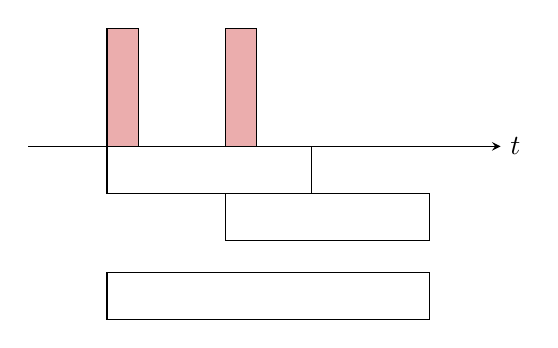
\begin{tikzpicture}
         \draw[-stealth] (0,0) -- (6,0) node[right] {$t$};
         \draw[fill=gray!40!red!40!] (1,0) rectangle ++ (0.4cm, 1.5cm);
         \draw[fill=gray!40!red!40!] (2.5,0) rectangle ++ (0.4cm, 1.5cm);
         \draw (1,0) rectangle ++ (2.6cm, -0.6cm);
         \draw (2.5,-0.6) rectangle ++ (2.6cm, -0.6cm);
         \draw (1,-1.6) rectangle ++ (4.1cm, -0.6cm);
      \end{tikzpicture}
   \end{figure}
\end{itemize}

Nel momento in cui si verifica il primo evento inizia la finestra di tempo morto e se durante tale intervallo arriva un secondo evento il tempo morto viene esteso. Se dovesse arrivare un terzo evento, il tempo morto si estenderà ancora e così via se ne dovessero arrivare altri. 

\subsection{Correzioni per il tempo morto}

Ci chiediamo adesso come fare per valutare qual è l'effetto del tempo morto in un sistema sul numero di conteggi. In altre parole, ci chiediamo come facciamo a capire se, dato che il sistema ha un suo tempo morto, il numero di conteggi che abbiamo misurato corrisponde alla frequenza di conteggio vera o se abbiamo perso degli eventi.

Sia $R_{\rm mis}$ il rate misurato cioè la frequenza di conteggio misurati, $R_{\rm vero}$ il rate vero e $\tau$ il tempo morto. Si può dimostrare che
\begin{itemize}[leftmargin=0.5cm]
   \item Nel caso di un rivelatore non paralizzabile la frequenza di conteggio vera è legata alla frequenza di conteggio misurata attraverso la relazione
   \begin{equation*}
      R_{\rm vero}=\frac{R_{\rm mis}}{1 + R_{\rm mis} \tau}
   \end{equation*}
   Attraverso questa, conoscendo il tempo morto e avendo misurato una certa frequenza di conteggio, possiamo calcolare il rate vero. Chiaramente, man mano che aumenta il tempo morto, $R_{\rm vero}$ e $R_{\rm mis}$ si discosteranno sempre più;
   \item nel caso di un rivelatore paralizzabile la relazione è più complessa, ed è la seguente:
   \begin{equation*}
      R_{\rm mis}=R_{\rm vero}e^{-R_{\rm vero} \tau}
   \end{equation*}
   la quale va risolta attraverso dei metodi iterativi.
\end{itemize}
Per entrambe le tipologie di rivelatore nel caso in cui la frequenza di conteggio è bassa, cioè quando $R_{\rm vero} \ll 1/\tau$, è valida l'approssimazione
\begin{equation*}
   R_{\rm mis}=R_{\rm vero}\bigl( 1 - R_{\rm vero} \tau \bigr)
\end{equation*}
Vediamo alcuni esempi numerici, in modo da quantificare l'effetto del tempo morto:

\begin{esempio}[Tempo morto di 10 microsecondi]
   Nella seguente tabella troviamo le perdite di conteggi nel caso in cui $\tau=10 \; \rm \mu s$ per sorgenti aventi rate via via crescenti.
   \begin{center}
      \begin{tabular}{p{2cm}p{3cm}p{2.5cm}}
         $R_{\rm mis}$ (Hz) & $R_{\rm vero}$ (Hz) & Perdite (\%)\\
         10 & 10,001 & 0,01\\
         100 & 100,1001 & 0,1\\
         1000 & 1010.101 & 1\\
         2000 & 2040,816 & 2\\
         3000 & 3092,784 & 3\\
         4000 & 4166,667 & 4\\
         5000 & 5263,158 & 5
      \end{tabular}
   \end{center}
   Notiamo come nel caso di rate bassi, ad esempio 10 particelle al secondo, un tale tempo morto non fa perdere quasi nulla, in quanto la probabilità che due eventi consecutivi si distanzino temporalmente meno di $10 \; \rm \mu s$ è bassissima dato che in media sono separate da $0.1$ s.\\
   Aumentando il rate l'effetto di perdita diventa più consistente, ad esempio con un rate di $5 \cdot 10^3 \; \rm Hz$ perdiamo il 5\% degli eventi.
\end{esempio}

\begin{esempio}[Tempo morto di 100 microsecondi]
   \E chiaro che se il tempo morto è più grande, le perdite nel conteggio saranno maggiori. Guardiamo i valori ottenuti nel caso di $\tau=100 \; \rm \mu s$:
   \begin{center}
      \begin{tabular}{p{2cm}p{3cm}p{2.5cm}}
         $R_{\rm mis}$ (Hz) & $R_{\rm vero}$ (Hz) & Perdite (\%)\\
         10 & 10,01001 & 0,1\\
         100 & 101,0101 & 1\\
         1000 & 1111.111 & 10\\
         2000 & 2500 & 20\\
         3000 & 4285,714 & 30\\
         4000 & 6666,667 & 40\\
         5000 & 10000 & 50
      \end{tabular}
   \end{center}
   Notiamo come per valori di rate elevato si arrivi a perdere fino al 50\% dei conteggi!
\end{esempio}

Vediamo adesso graficamente l'andamento del rate misurato in funzione del rate vero, indicati nel grafico seguente rispettivamente con $m$ e $n$:
\begin{figure}[H]
   \centering
   \includegraphics[width=0.7\textwidth]{immagini/rate_vero_e_rate_misurato.png}
\end{figure}
Notiamo come nel caso ideale in cui $R_{\rm vero}=R_{\rm mis}$ tale grafico coincide con la prima bisettrice. Nella realtà ci sono delle perdite dovute al tempo morto, le quali dipendono ovviamente dal rate (notiamo come per bassi valori di questo le curve praticamente coincidano) ma soprattutto dipendono dal modo di funzionamento del rivelatore, cioè se è paralizzabile o non paralizzabile. Nel caso non paralizzabile si ha una perdita abbastanza limitata, mentre nel caso paralizzabile, a causa del fatto che il sistema si paralizza perché il tempo morto viene esteso sempre più man mano che arrivano particelle durante la stessa finestra temporale, il rivelatore può perdere quasi tutte le particelle che arrivano e dunque le perdite sono più incidenti.

Guardiamo adesso un grafico simile al precedente ma relativo soltanto al caso di rivelatore non paralizzabile, dove le varie curve sono ottenute per valori di tempo morto differenti:

\begin{figure}[H]
   \centering
   \includegraphics[width=0.6\textwidth]{immagini/rate_vero_e_rate_misurato_caso_non_paralizzabile.png}
\end{figure}

Notiamo come, all'aumentare del tempo morto, le curve si discostano sempre più dalla bisettrice, il che indica che la perdita di eventi è maggiore.

\subsection{Come stimare il tempo morto?}

A volte il tempo morto viene fornito dal costruttore, ma se non avessimo a disposizione questa informazione questo si può misurare sperimentalmente.

\begin{esempio}[Metodo delle due sorgenti]
   Esistono diverse tecniche per valutare il tempo morto, in particolare una tecnica molto adoperata è il cosiddetto metodo delle due sorgenti, che consiste nell'adoperare un rivelatore e nel posizionare in due posizioni fisse delle sorgenti come in figura
   \begin{figure}[H]
      \centering
      \begin{tikzpicture}[>=stealth,shorten >=1.8pt,shorten <=1.8pt,]
         \node at (0,0) [thick,red!40!gray,cylinder, shape border rotate=90, draw,minimum height=3cm,minimum width=2cm,cylinder uses custom fill, cylinder end fill=gray!25!red!50!, cylinder body fill=gray!25!red!30!,rotate=90,shape aspect=4] {};
         \node at (-4,-0.8) [thick,teal!40!gray,cylinder, shape border rotate=90, draw,minimum height=0.5cm,minimum width=1cm,cylinder uses custom fill, cylinder end fill=gray!25!teal!50!, cylinder body fill=gray!25!teal!30!,rotate=90,shape aspect=2] {};
         \node at (-4,0.8) [thick,teal!40!gray,cylinder, shape border rotate=90, draw,minimum height=0.5cm,minimum width=1cm,cylinder uses custom fill, cylinder end fill=gray!25!teal!50!, cylinder body fill=gray!25!teal!30!,rotate=90,shape aspect=2] {};
         \node[above=1.5cm] at (-4.2,0) {Sorgenti};
         \node[above=1.5cm] at (-0.2,0) {Rivelatore};
      \end{tikzpicture}
    \end{figure}
   I passi di tale metodo sono i seguenti:
   \begin{enumerate}[leftmargin=0.5cm]
      \item Misura con la prima sorgente: Si utilizza una sorgente radioattiva e si misura il numero di conteggi per unità di tempo ($R_1$) registrati dal rivelatore;
      \item Misura con la seconda sorgente: Si utilizza una seconda sorgente radioattiva, che deve essere indipendente dalla prima, e si misura il numero di conteggi per unità di tempo ($R_2$);
      \item Misura con entrambe le sorgenti: Si posizionano entrambe le sorgenti vicine al rivelatore e si misura il numero di conteggi totali per unità di tempo ($R_{12}$).
   \end{enumerate}
   Il numero di conteggi attesi $R_{12}$ quando entrambe le sorgenti sono attive dovrebbe essere approssimativamente la somma dei conteggi singoli ($R_1 + R_2$) se non ci fosse tempo morto. Tuttavia, a causa del tempo morto, il numero di conteggi osservato $R_{12}$ sarà inferiore. In base al rate misurato si può stimare il tempo morto tramite la relazione
   \begin{equation*}
      \tau=\frac{R_1R_2 - \sqrt{R_1R_2( R_{12} - R_1 )( R_{12} - R_2 )}}{R_1R_2R_{12}}
   \end{equation*}
   Tale metodo è abbastanza semplice da adoperare, ma ha delle difficoltà che dipendono
   \begin{itemize}[leftmargin=0.5cm]
      \item dalla statistica che andiamo a misurare, perché è tanto più preciso quanto più è lunga la misura che effettuiamo, in quanto le fluttuazioni statistiche diventano sempre meno importanti man mano che aumenta la statistica;
      \item dalla capacità dello sperimentatore di posizionare le sorgenti nello stesso punto, in quanto tra la misure di un rate e dell'altro le sorgenti vanno spostate per poi essere poste nella stessa posizione.
   \end{itemize}
\end{esempio}

\section{Funzioni di un rivelatore}

Oltre ad informazioni su energia e tempo di volo, a seconda della tipologia di rivelatore, è possibile avere accesso ad altre informazioni sulle particelle che incidono. Ad esempio, oltre all'energia, si potrebbe misurare:

\begin{itemize}
   \item l'impulso, che grossomodo ad alte energie (cioè energie molto più grandi della massa a riposo della particella) dà un'informazione sull'energia della particella;
   \item carica;
   \item massa
   \item tempo di arrivo.
\end{itemize}

In generale, per avere accesso a tutte le informazioni, poiché è impossibile che un unico rivelatore fornisca tutte le informazioni si adoperano grandi sistemi di rivelazione, costituiti da diversi sotto-rivelatori che sfruttano tecnologiche diverse. I grandi rivelatori per la fisica nucleare/particellare comprendono diverse componenti (sotto-rivelatori) per il tracciamento e l'identificazione delle numerose (anche decine di migliaia) particelle prodotte in una singola collisione.

Ad esempio, quando si esplorano regimi di energia molto elevati come le collisioni tra fasci di particelle a energia molto elevata, quello che succede è che da queste collisioni vengono emesse tantissime particelle e di conseguenza i rivelatori che bisogna adoperare sono estremamente complessi, in quanto devono essere in grado di misurare tutte le particelle emesse dal punto di interazione, e in tal caso è necessario una geometria a $4\pi$ che normalmente viene assicurata con geometrie cilindriche che avvolgono il punto di interazione più degli end-tap, cioè dei rivelatori che vanno a fare da "tappo" alle estremità. Quindi non serve solo un'efficienza il più possibile prossima 100\%, ma anche delle tecnologie che permettono di capire le diverse tipologie di particelle che sono state prodotte per andare a studiare diversi segnali. 

Come questi sistemi di rivelazione effettuano queste operazioni è un punto abbastanza complesso, in quanto essi devono saper ricostruire le tracce delle particelle, quindi alcuni di questi devono essere dei rivelatori di tracciamento, cioè in grado di andare a visualizzare in qualche modo il passaggio delle particelle e andare a tracciare delle linee che rappresentano il percorso seguito da diverse particelle;inoltre essi devono essere in grado di identificare le particelle oppure essere in grado di rivelare fotoni di alta energia.

\subsection{Misura dell'energia}

Uno dei compiti dei rivelatori è misurare l'energia, che come abbiamo già accennato è un aspetto importante soprattutto quando si vanno a misurare elettroni o fotoni di alta energia, perché in quei casi si producono degli sciami elettromagnetici e per misurare l'energia del gamma/elettrone di partenza è necessario adoperare dei rivelatori in grado di contenere eventuali sciami che si sviluppano.

I rivelatori che vanno a misurare l'energia totale di una particella o di una radiazione sono detti calorimetri. Un esempio di tali rivelatori sono i calorimetri elettromagnetici/adronici, usati soprattutto nella fisica delle alte energie.

\subsection{Misura dell'impulso}
Un'altra tecnica per misurare l'energia di particelle cariche è quella di andare a misurare l'impulso, perché questa in pratica è una misura dell'energia.

Tale misura si effettua curvando la particella mediante un opportuno campo magnetico, sfruttando la forza di Lorentz e andando a produrre delle traiettorie circolari o elicoidali. Conoscendo poi il raggio di curvatura è possibile risalire all'impulso.

Bisogna tenere conto del fatto che i valori di energia che si devono misurare possono essere molto diversi tra loro: si va da pochi meV fino a $10^{20}$ eV nel caso dei raggi cosmici di alta energia, per cui le tecnologie che si devono adoperare di differiscono a seconda del valore di energia che si vuole misurare.

Nella fisica nucleare di bassa energia si utilizzano opportuni spettrometri magnetici, esistenti sotto varie configurazioni e il cui utilizzo consente una risoluzione in impulso estremamente elevata.

Per deflettere una particella carica e misurarne l'impulso dalla curvatura della traccia si può usare un dipolo magnetico come in figura:

\begin{figure}[H]
   \centering
   \includegraphics[width=0.6\textwidth]{immagini/dipolo_magnetico_impulso.png}
\end{figure}

Un altro esempio di magnete, usato per deflettere le particelle cariche prodotte in una reazione nucleare di un fascio con un target fisso può essere il seguente:

\begin{figure}[H]
   \centering
   \includegraphics[width=0.6\textwidth]{immagini/magnete_misura_impulso.png}
\end{figure}

\subsection{Misura della carica/massa}

Una particella può essere identificata anche sfruttando la perdita di energia in un rivelatore, perché la formula di Bethe-Bloch non dipende soltanto dalle caratteristiche del materiale che viene investito (in questo caso del rivelatore) ma anche dalle caratteristiche della particella. \E quindi possibile andare a discriminare le diverse tipologie di particelle a seconda della perdita di energia che hanno all'interno del rivelatore, dunque il base al segnale che producono.

In figura possiamo vedere tipiche curve che si ottengono, che richiamano la forma della curva di Bethe-Bloch:

\begin{figure}[H]
   \centering
   \includegraphics[width=0.6\textwidth]{immagini/grafici_perdita_energia.png}
\end{figure}

Un andamento del genere è chiamato dai fisici "a banana" ed è in particolare l'andamento iniziale della curva di Bethe-Bloch, il quale ha un andamento iperbolico.

Nel grafico si osservano diverse distribuzioni di punti in corrispondenza di diverse tipologie di particelle. Chiaramente i punti non si dispongono esattamente su una linea ma si addensano di più in corrispondenza di un determinato pattern in questo grafico, e ciò è dovuto a effetti di risoluzione in energia che fanno discostare i valori misurati sperimentalmente dalla curva ideale.